\documentclass{beamer}

\usepackage[latin1]{inputenc}
\usepackage{graphicx}
\usepackage{amsmath,amssymb,amsthm}
\usepackage[mathscr]{eucal}
\usepackage{textcomp}
\usepackage{subfig}
\usepackage{epsfig}
\usepackage{multirow}
\usepackage{hhline}
\usepackage{bm}
\usefonttheme[onlymath]{serif}

\beamertemplatetextbibitems

\usetheme{Boadilla}
\usecolortheme{seahorse}

%% Footnote for Figures
\newcommand\blfootnote[1]{%
   \begingroup
   \renewcommand\thefootnote{}\footnote{#1}%
   \addtocounter{footnote}{-1}%
   \endgroup
}

\usepackage[latin1]{inputenc}

\title[CinC 2020]{Tensor-Based Noninvasive Atrial Fibrillation Complexity Index For Catheter Ablation} 
\author[Lucas de S. Abdalah]{\textbf{Lucas de S. Abdalah}, Pedro Marinho R. de Oliveira, Walter Freitas Jr,\\Vicente Zarzoso}
\date{Sep 16{\textsuperscript{th}}, 2020}

\begin{document}
%% ------------------------- Title --------------------------------------------
	\begin{frame}
		\begin{figure}[!htb]
			\centering
			
\includegraphics[scale=0.055]{UCA_logo} 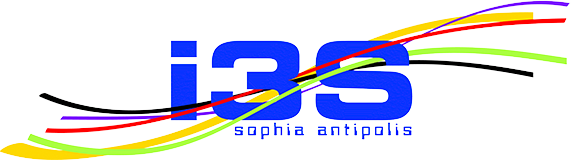
\includegraphics[scale=0.150]{I3S_logo} 
\includegraphics[scale=0.025]{CNRS_logo.png} 
\includegraphics[scale=0.130]{UFC_logo.png}
		\end{figure}
		\vspace{-0.4cm}

		\titlepage
	\end{frame}

%% ------------------------- Introduction -------------------------------------
\section{Introduction} 
	
	\begin{frame}
		\frametitle{Atrial Fibrillation}	
		
		\begin{itemize}
			\item Atrial Fibrillation (AF) is the most common sustained cardiac arrhythmia encountered in clinical practice.
			\begin{itemize}
				\item  In the EU, the number of adults with AF will double from 2010 to 2060\footnote{Krijthe \textit{et al}., ``Projections on the number of individuals with atrial fibrillation in the European Union, from 2000 to 2060,'' \textit{Eur Heart J}. 2013.}.
			\end{itemize}
		\end{itemize}
		\begin{figure}
			\centering
			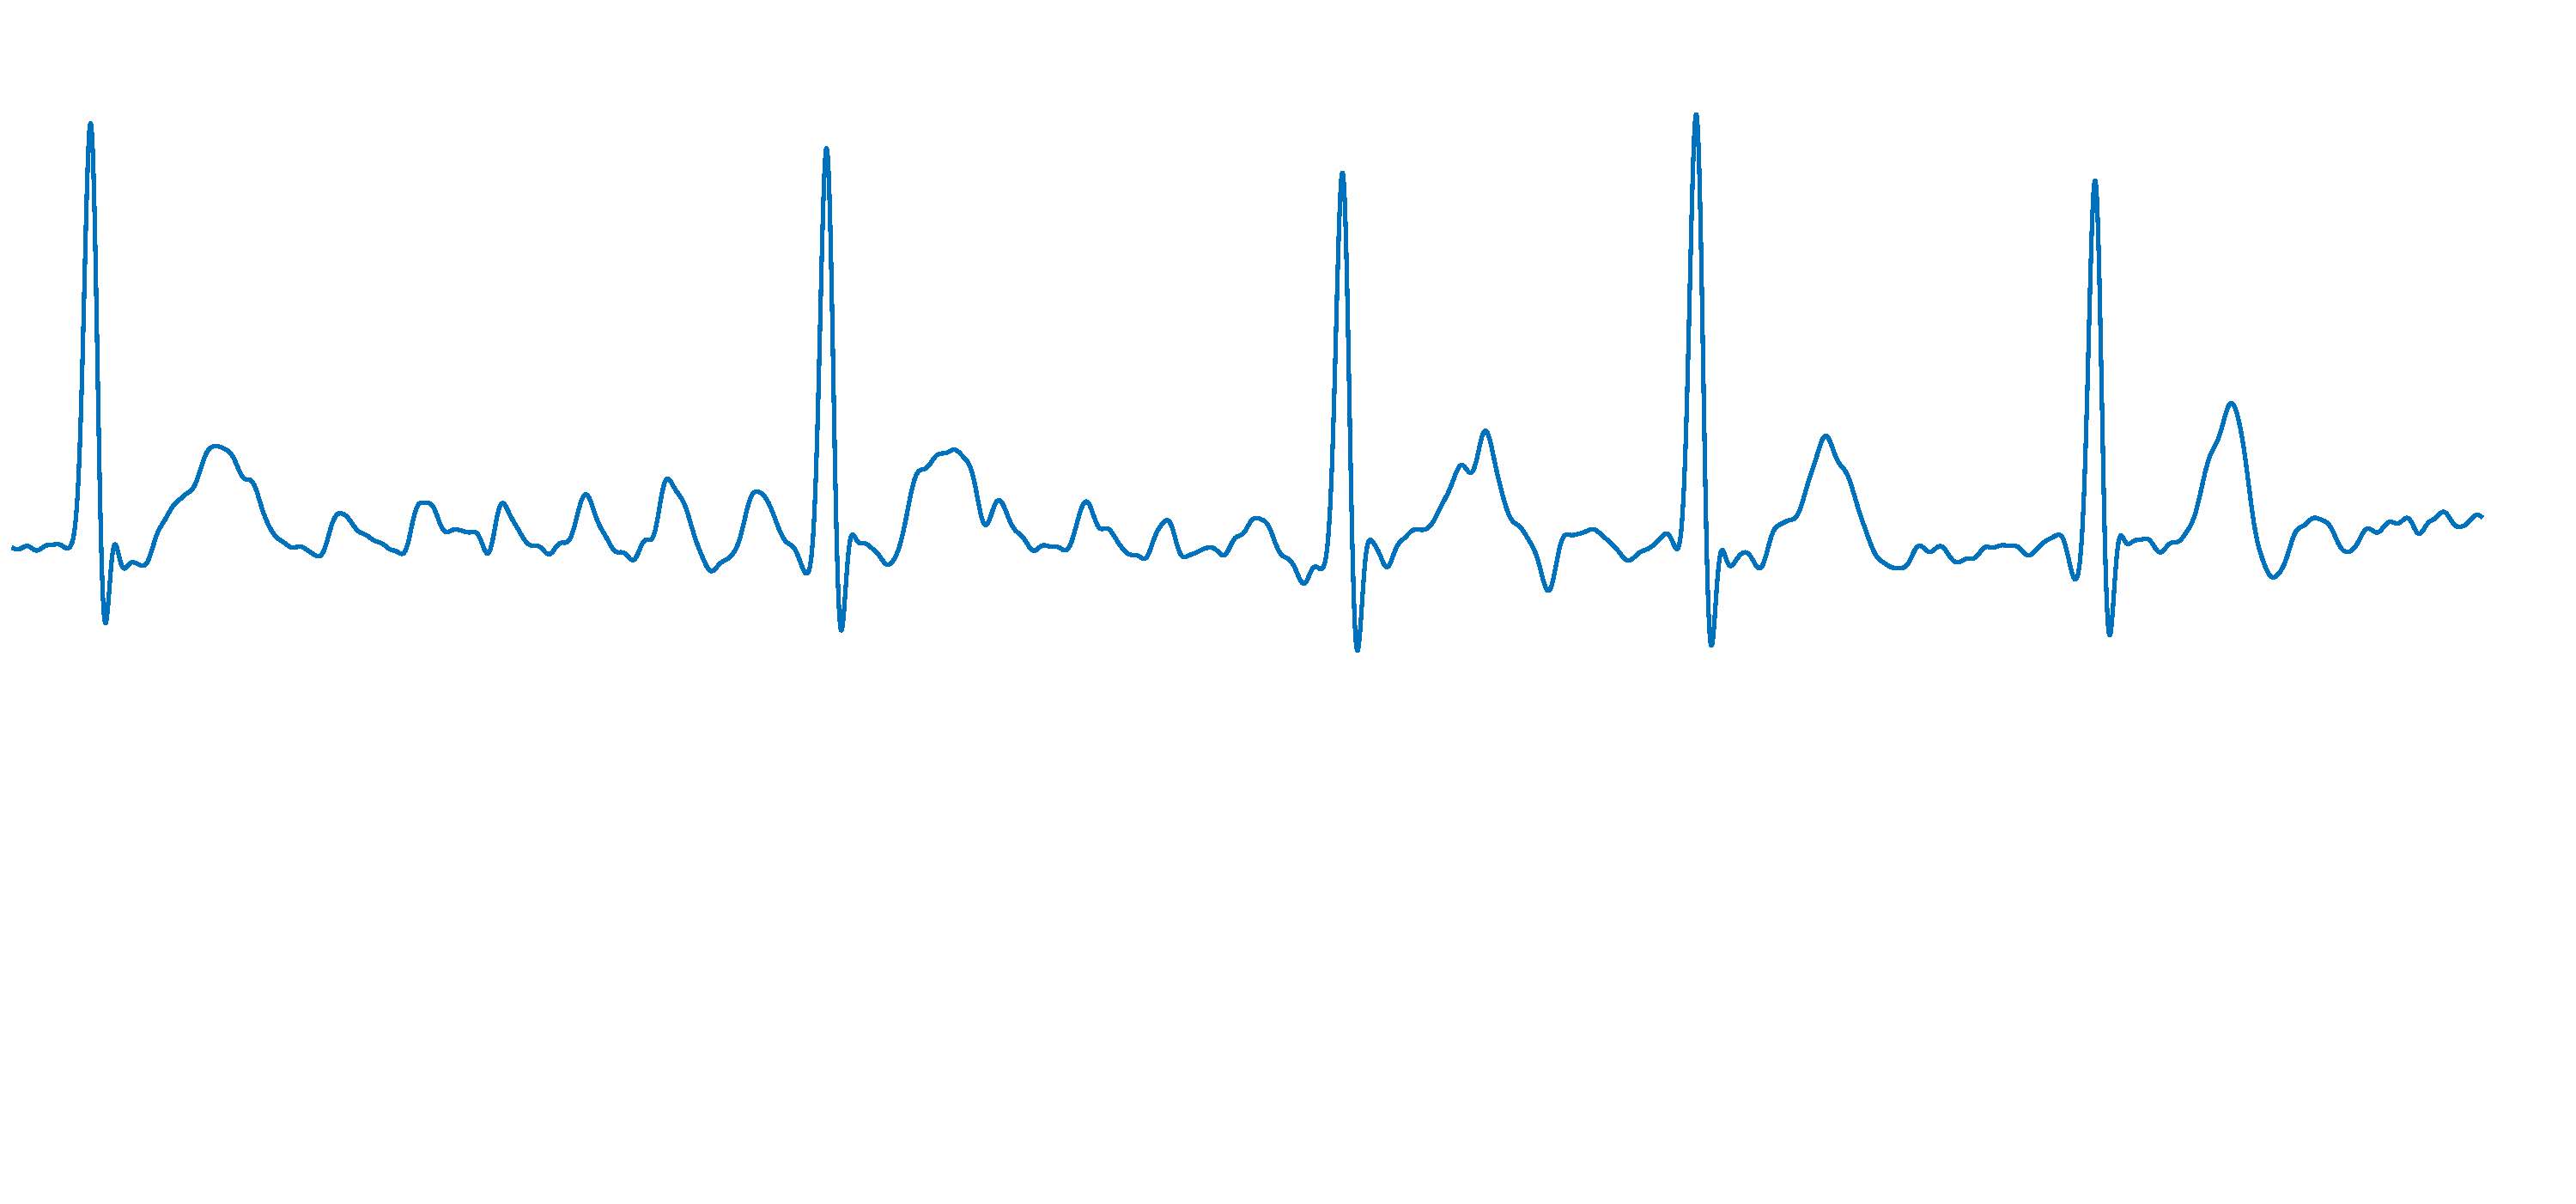
\includegraphics[scale=0.2]{AF_ECG-eps-converted-to.pdf}
		\end{figure}
		\vspace{-0.8in}	
		\begin{itemize}
			\item The complex electrophysiological mechanisms underlying AF are not completely understood.
		\end{itemize}
	\end{frame}

	\begin{frame}
		\frametitle{Step-wise Catheter Ablation (CA)}
		
		\begin{figure}[h]
			\centering
			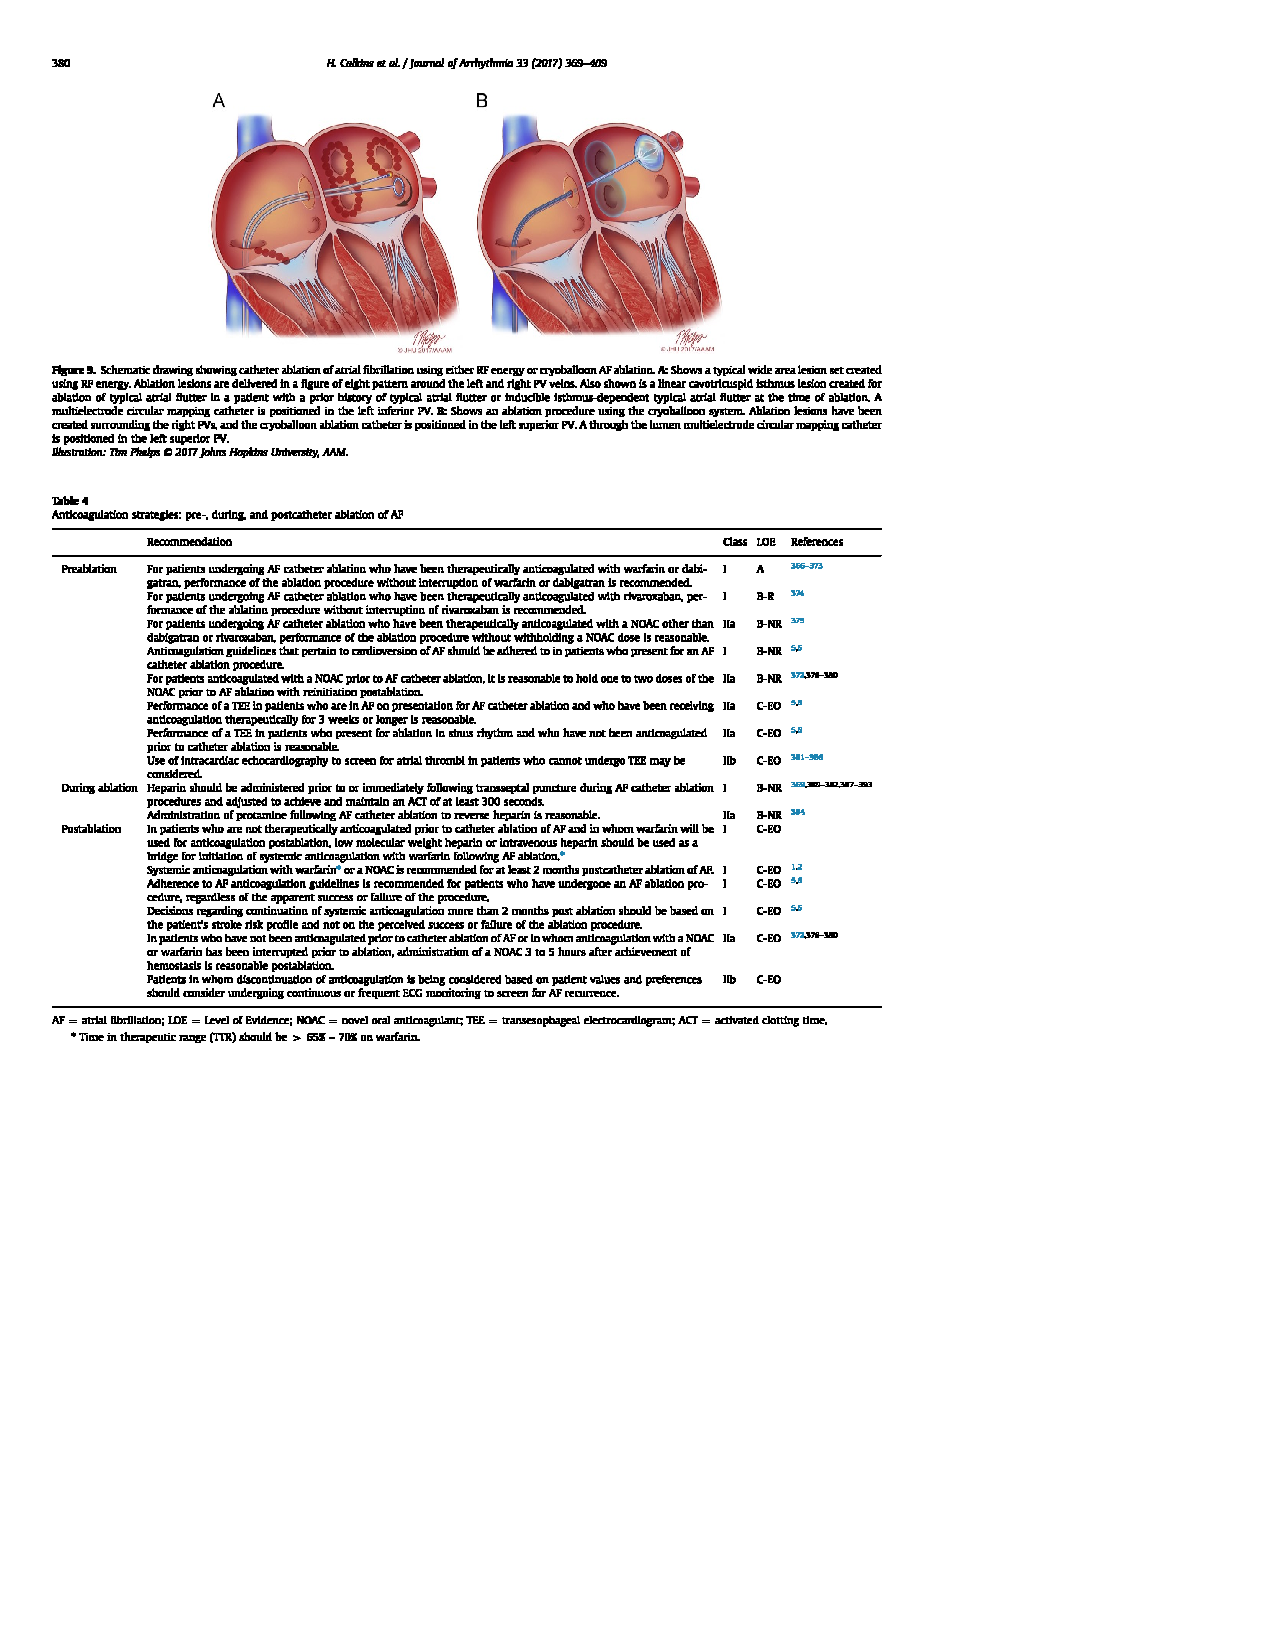
\includegraphics[scale=1.2,clip=true,trim={3.55cm 21.95cm 13.8cm 2.0cm}]{CA_figure.pdf}
		\end{figure}
		\blfootnote{Figure from Tim Helps $^{\text{\tiny{\copyright}}}$ 2017 Johns Hopkins University, AAM}
		\vspace{-0.8cm}
		\begin{itemize}
			\item Noninvasive techniques to assess AF electrophysiological complexity can help guide step-wise CA in real time.
			\begin{itemize}
				\item Impact of pulmonary vein isolation (PVI) and other widely used techniques on atrial activity (AA) complexity.
			\end{itemize}
		\end{itemize}
	\end{frame}

	\begin{frame}
		\frametitle{Matrix Approach}
	
		The ECG data matrix can be modeled as:
		\begin{equation}
			\textbf{Y} = \textbf{MS} \in \mathbb{R}^{K \times N} \; ,
		\end{equation}
		where ${\textbf{M}} \in {\mathbb{R}}^{K \times R}$ is a mixing matrix and $\textbf{S} \in {\mathbb{R}}^{R \times N}$ is the source matrix.	
		\vspace{-0.4cm}
		\begin{figure}[htb]
			\centering
			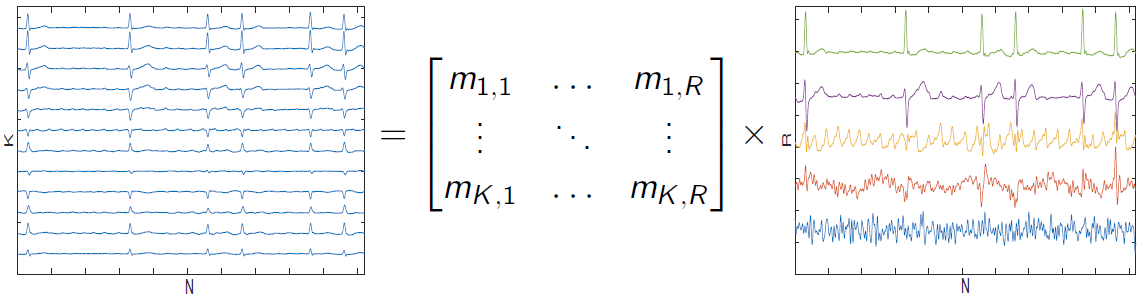
\includegraphics[scale=0.5]{bss_fig.png}
		\end{figure}
	\end{frame}
		
%% ------------------------- Methods ------------------------------------------
\section{Methods}

	\begin{frame}
		\frametitle{Tensor Approach}
		
		\begin{itemize}
			\item The ECG data can be modeled as a 3rd-order tensor ${\mathcal{Y}}$ via row-Hankelization.
			\begin{itemize}
				\item Tensor decompositions factorize data as a sum of simpler tensors.
			\end{itemize}
		\end{itemize}
		\vspace{-0.7cm}
		\begin{figure}[htb]
			\centering
			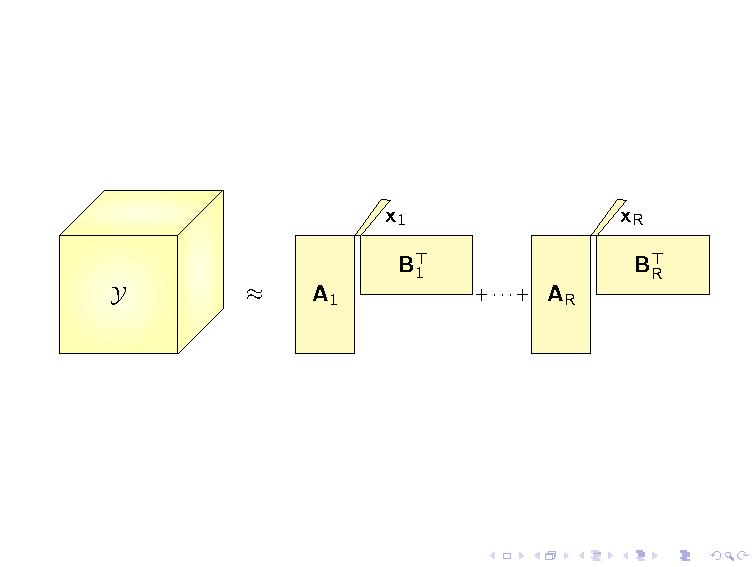
\includegraphics[scale=0.8,clip=true,trim={0.8cm 6.5cm 0.6cm 6.2cm}]{tikz_BTDY.pdf}
		\end{figure}
		\vspace{2.3cm}
		\begin{itemize}
			\item Block Term Tensor Decomposition (BTD) based on Hankel structure\footnote{De Lathauwer, ``Blind separation of exponential polynomials and the decomposition of a tensor in rank-($L_{r}$,$L_{r}$,1) terms,'' \textit{SIAM J. Matrix Anal. Appl.}, 2011.}.
		\end{itemize}
	\end{frame}
		
	\begin{frame}
		\frametitle{BTD-Hankel Model}
		
		\vspace{-0.5cm}
		\begin{block}{Low-rank Hankel structure}
			\begin{itemize}
				\item AA signal during AF can be represented by an all-pole model (2)
			\end{itemize}
			\begin{itemize}
				\item The structured Hankel matrix has a rank equal to the number of poles ($L_{r}$)
			\end{itemize}
		\end{block}
		\begin{columns}
			\begin{column}{0.5\textwidth}		
				\vspace{2.5cm}
				\begin{equation}
					s(n) = \sum_{\ell = 1}^{L_{r}} \alpha_{\ell} z_{\ell}^{n}
				\end{equation}
			\end{column}
			\begin{column}{0.5\textwidth}
				\begin{figure}[htb]
					\vspace{-5.0cm}
					\centering
					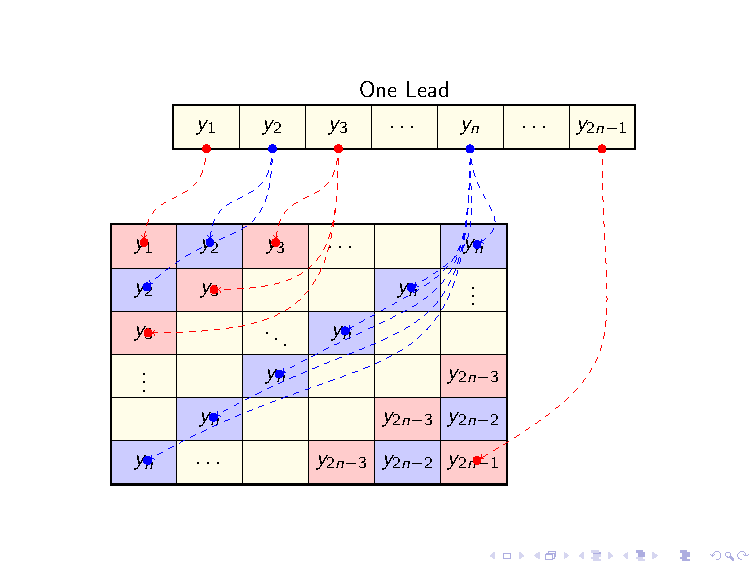
\includegraphics[scale=0.66,clip=true,trim={1.5cm 8.5cm 1.8cm 8.3cm}]{tikz_mapHankel.pdf}
				\end{figure}
			\end{column}
		\end{columns}
	\end{frame}

	\begin{frame}
		\frametitle{Tensor Approach}
		
		\vspace{-3.5cm}
		\begin{itemize}
			\item Stack each Hankel matrix in the 3rd-mode of the tensor $\mathcal{Y}$.
		\end{itemize}
		
		\vspace{3.0cm}
		\begin{figure}[!ht]
			\centering
			\vspace{-3.5cm}
			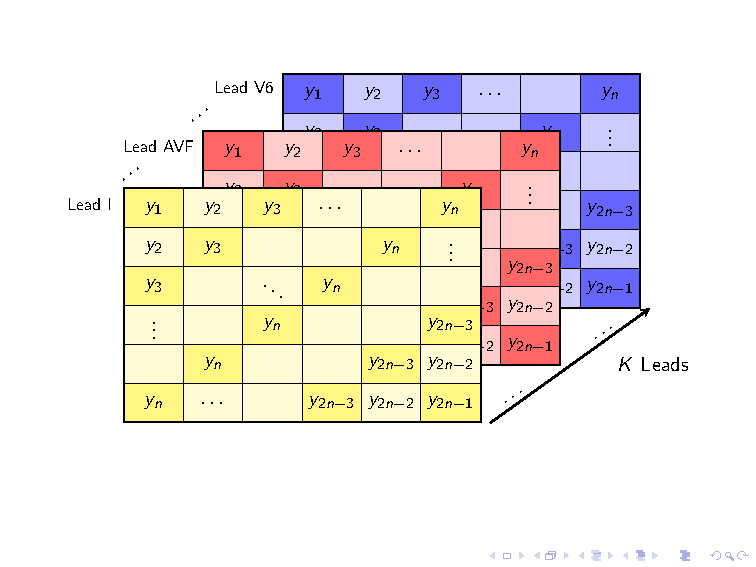
\includegraphics[scale=1.0,trim={1.0cm 8.5cm 1.0cm 7.3cm},clip=true]{tikz_tensorHankel.pdf}
		\end{figure}
	\end{frame}

	\begin{frame}
		\frametitle{BTD Approach}
		
		\vspace{-0.7cm}
		\begin{figure}[htb]
			\centering
			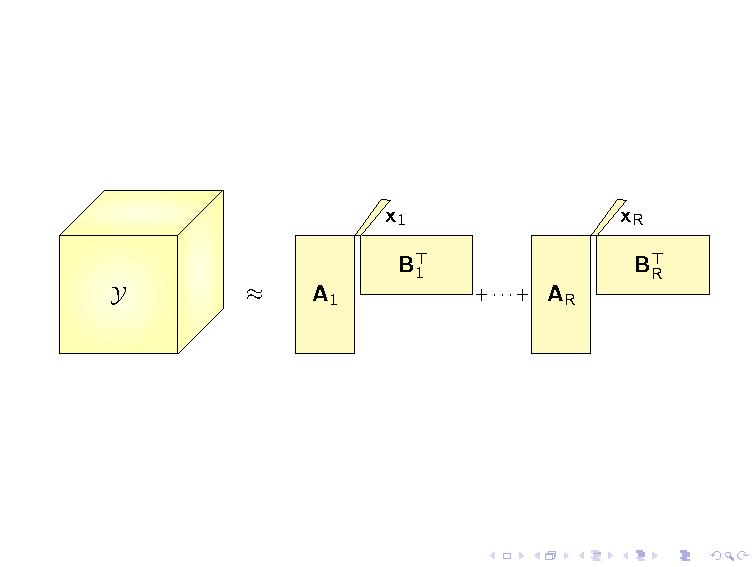
\includegraphics[scale=1.0,clip=true,trim={0.8cm 6.5cm 0.6cm 6.2cm}]{tikz_BTDY.pdf}
		\end{figure}
		\vspace{2.8cm}
		\begin{block}{Challenge}			
				\begin{itemize}
					\item Parameter estimation
					\begin{itemize}
						\item $R$, $L_{r}$
					\end{itemize}
					\item Factor estimation
					\begin{itemize}
						\item $\textbf{A}$, $\textbf{B}$, $\textbf{X}$
					\end{itemize}
				\end{itemize}
		\end{block}
	\end{frame}

	\begin{frame}
		\frametitle{Constrained Alternating Group Lasso}
		
		\begin{block}{Classical BTD Approach}
			\begin{itemize}
				\item Fixed structure minimizing $f(\textbf{A}, \textbf{B}, \textbf{X})$ with prior knowledge of $(R,L_{r})$
			\end{itemize}
		\end{block}
		\begin{equation}
			f(\textbf{A}, \textbf{B}, \textbf{X}) \triangleq
			 \Big\| {\mathcal{Y}} - \textstyle \sum_{r = 1}^{R} \left( \textbf{A}_r \textbf{B}_r^{\top} \right) \circ \textbf{x}_r  \Big\|_F^2
		\end{equation}
		\begin{block}{Constrained Alternating Group Lasso (CAGL) Approach}
			\begin{itemize}
				\item Non-fixed structure minimizing $F(\textbf{A},\textbf{B},\textbf{X})$ ensuring the Hankel structure
				\item Penalization term ($\gamma$) and $g({\textbf{A}, \textbf{B}, \textbf{X}})$ limiting the multilinear ranks and number of blocks
				\item Allows simultaneous estimation of $(R,L_{r})$ and model factors
			\end{itemize}
		\end{block}
		\begin{equation}
				  F({\textbf{A}, \textbf{B}, \textbf{X}})
				 \triangleq  
				 f({\textbf{A}, \textbf{B}, \textbf{X}}) + \gamma \, g({\textbf{A}, \textbf{B}, \textbf{X}})
		\end{equation}
	\end{frame}
	
	\begin{frame}
		\frametitle{AF Complexity Index}
		
		\begin{block}{Signal Complexity}
			The more poles the signal contains, the more complex it can be considered
		\end{block}
		
		\begin{itemize}
			\item The complexity index proposed in this work is based on the number of poles $L_{r}$ contained in a signal. 
			\item The Hankel matrix rank is equal to number of poles $L_{r}$.
		\end{itemize}

	\end{frame}
	
	\begin{frame}
		\frametitle{Atrial Source Classification}
			
			\begin{block}{Challenge}
				After performing CAGL, the automated AA source classification is still a problem
			\end{block}
			
			\begin{itemize}
				\item Spectral concentration (SC), dominant frequency (DF), kurtosis and visual inspection to evaluate AA extraction\footnote{De Oliveira and Zarzoso, ``Source analysis and selection using block term decomposition in atrial fibrillation'', in \textit{Proc. LVA/ICA}, 2018.}.
			\end{itemize}
	\end{frame}	

	\begin{frame}
		\frametitle{AA Source Estimation}
		
		\vspace{-1.5cm}
		\begin{figure}[!ht]
			\centering
			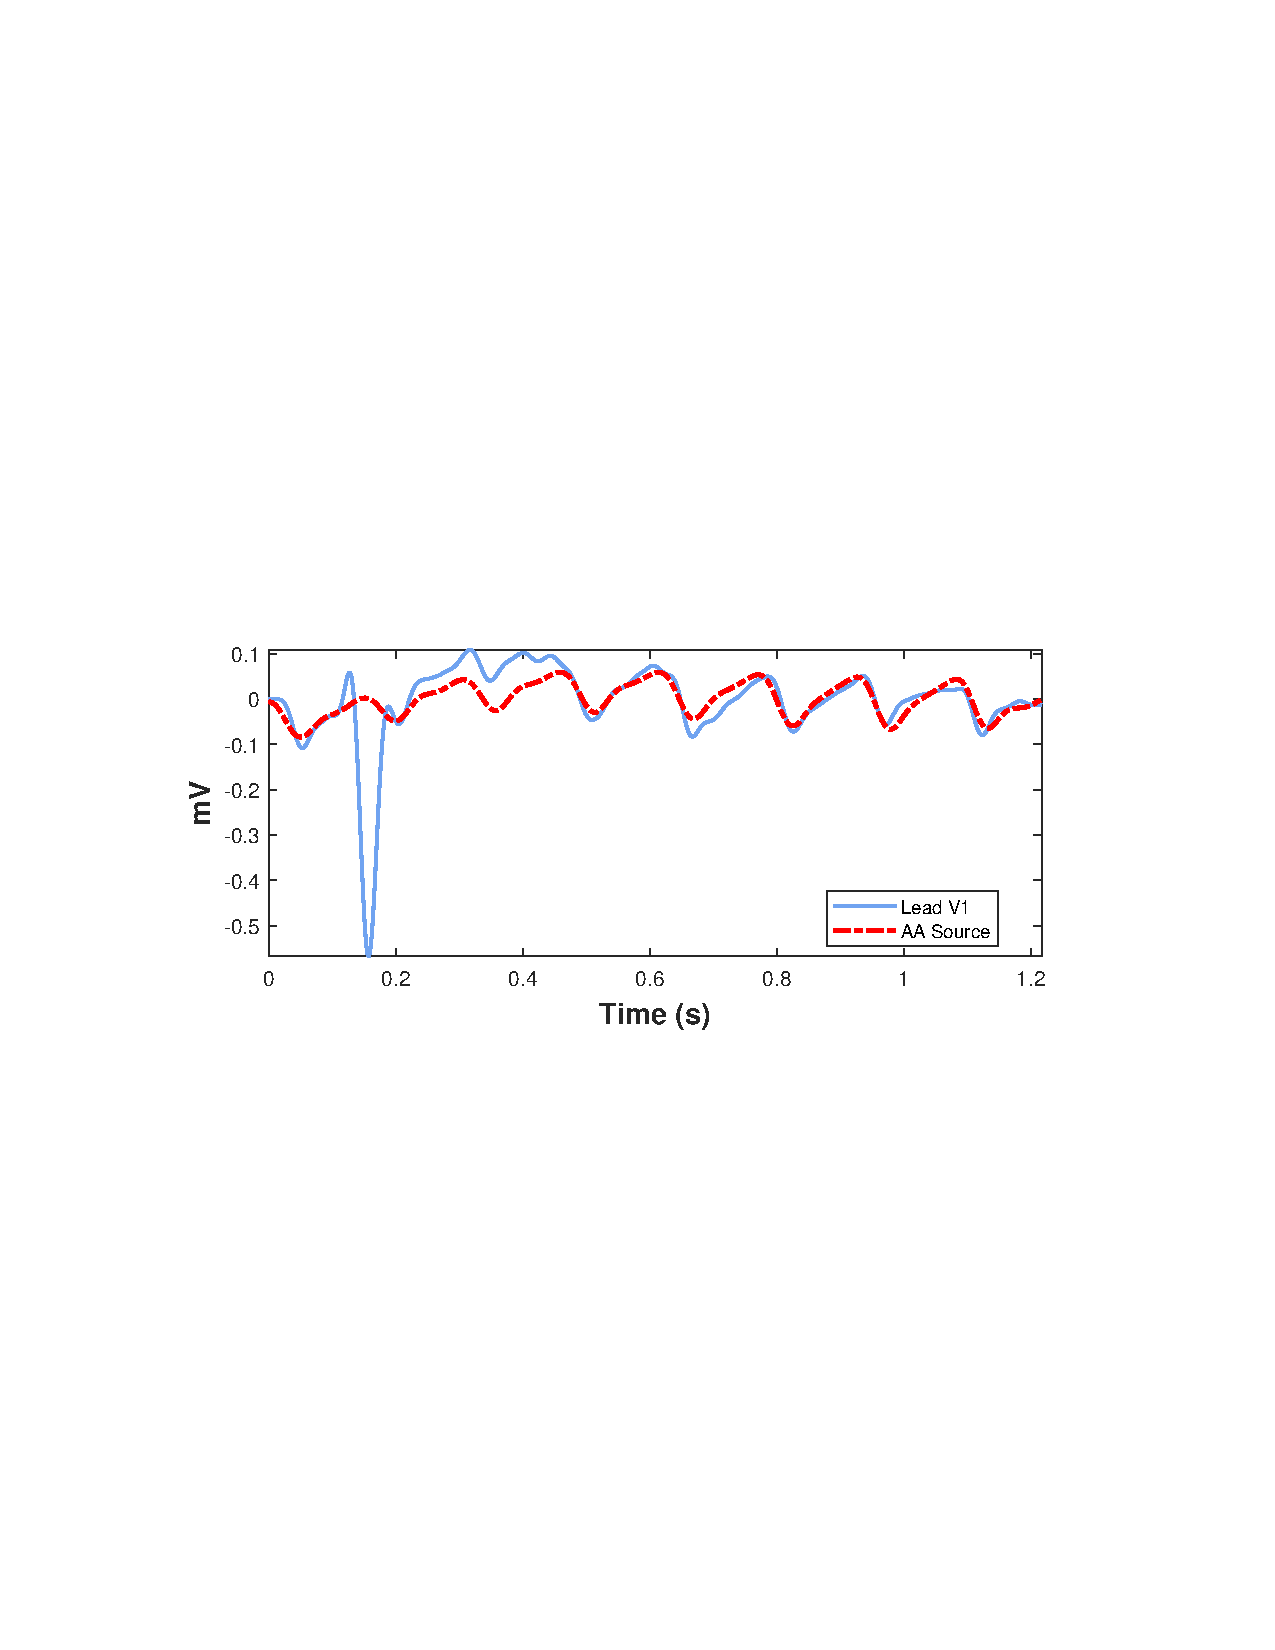
\includegraphics[scale=0.75,trim={3.0cm 8.5cm 3.0cm 8.5cm},clip=true]{example_Source.pdf}
		\end{figure}
		\vspace{-2.0cm}
		
		\begin{itemize}
			\item SC $=$ 74.3\%
			\item DF $=$ 6.4 Hz
			\item Kurtosis $=$ 177.0
			\item AA Hankel Matrix Rank $=$ 33
		\end{itemize}
		
	\end{frame}

%% ------------------------- Experimental Results -----------------------------
\section{Experimental Results}

	\begin{frame}
		\frametitle{Database and Experimental Setup} 
			
		\begin{block}{Database}
			\begin{itemize}
				\item 20 patients suffering from persistent AF
				\item 59 ECG segments from 0.72 to 1.42 seconds
			\end{itemize}
			
			\begin{center}
				Cardiology Department of Princess Grace Hospital Center, Monaco
			\end{center}					
		\end{block}	
		
		\begin{itemize}
			\item Hankel-based BTD was implemented using CAGL.
		\end{itemize}
	\end{frame}

	\begin{frame}
		\frametitle{Impact of CA step on AA complexity}
		
		\vspace{-0.5cm}
		\begin{figure}[h]
			\centering
			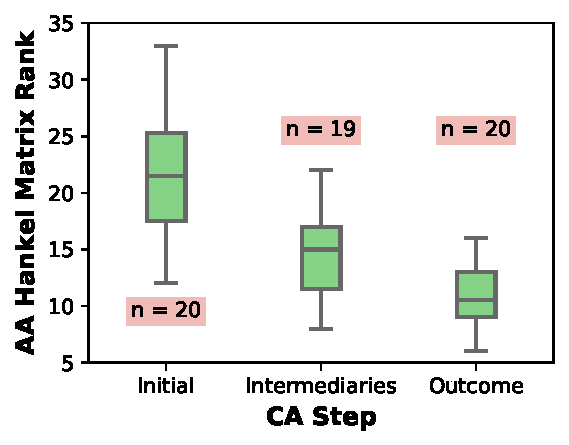
\includegraphics[scale=0.9]{boxplot_complexity.pdf}
		\end{figure}
		\vspace{-0.5cm}
		\begin{itemize}
			\item 20 patients undergoing various CA steps
			\item 59 ECG segments (1.06 $\pm$ 0.2 s)
		\end{itemize}
	\end{frame}

	\begin{frame}
		\frametitle{Impact of PVI on AA complexity}

		\vspace{-0.5cm}
		\begin{figure}[h]
			\centering
			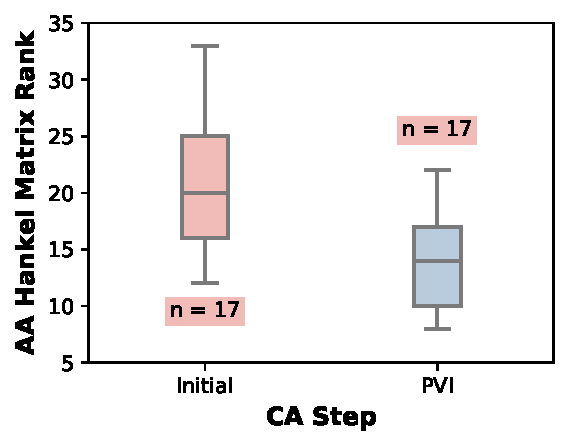
\includegraphics[scale=0.9]{boxplot_PVI.pdf}
		\end{figure}
		\vspace{-0.5cm}
		\begin{itemize}
			\item 17 patients undergoing PVI
			\item 34 ECG segments
		\end{itemize}
	\end{frame}

	\begin{frame}
		\frametitle{AF Recurrence vs. Complexity Before CA} 
		
		\vspace{-0.3cm}
		\begin{figure}[h]
			\centering
			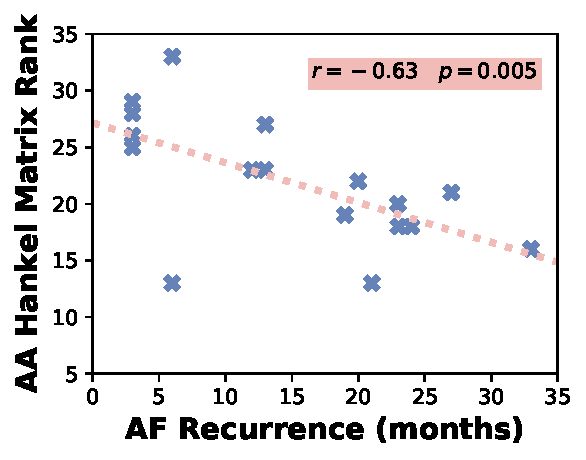
\includegraphics[scale=0.7]{rank_LR.pdf}
		\end{figure}
		\vspace{-0.5cm}
		\begin{block}{Relationship}
			A significant Pearson correlation between AF recurrence and the proposed index
			\begin{itemize}
				\item 18 patients with complete follow-up information
			\end{itemize}
		\end{block}	
	\end{frame}

%% ------------------------- Conclusion ---------------------------------------
\section{Conclusions}

	\begin{frame}
		\frametitle{Conclusions} 
		
		\begin{block}{Contributions}
			\begin{itemize}
				\item Jointly extract the AA signal and measure AF complexity via tensor decomposition
				\item Very short ECG recordings (1.06 $\pm$ 0.20 s)
				\item Validation in 20 patients undergoing CA
				\begin{itemize}
					\item Expected decreasing AF complexity throughout CA steps
					\item Significant correlation with AF recurrence after CA
				\end{itemize}
			\end{itemize}
		\end{block}
		
		\begin{block}{Clinical Impact}
			\begin{itemize}
				\item A potential tool to help guide CA in real time
			\end{itemize}
		\end{block}

		\begin{block}{Future Work}
			\begin{itemize}
				\item Increase number of patients in the database
				\item Compare the proposed index with other state-of-the-art indices
				% \item Automated source classification.
			\end{itemize}
		\end{block}
		
	\end{frame}
		
\end{document}